\section[Objectifs et approches]{Objectifs et approche du problème}

	\begin{frame}
		\begin{minipage}{0.47\textwidth}
			\begin{Vblock}{\only<1>{Ouvertures}\only<2>{Finales}}
				Pré-calculer tous les \only<1>{débuts\\}\only<2>{fins} possibles
			\end{Vblock}
			\begin{figure}
				\only<1>{
					\begin{minipage}{0.49\textwidth}
						\centering
						\textbf{A}
						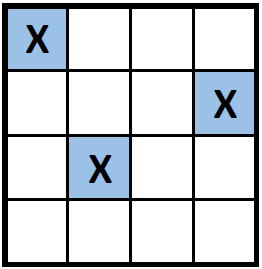
\includegraphics[width=\linewidth]{images/placement_random}
					\end{minipage}\hfill
					\begin{minipage}{0.49\textwidth}
						\centering
						\textbf{B}
						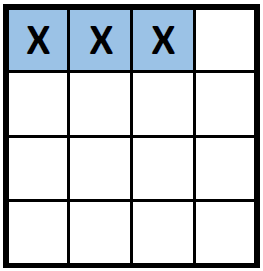
\includegraphics[width=\linewidth]{images/placement_rowscan}
					\end{minipage}\hfill
				}
				\only<2>{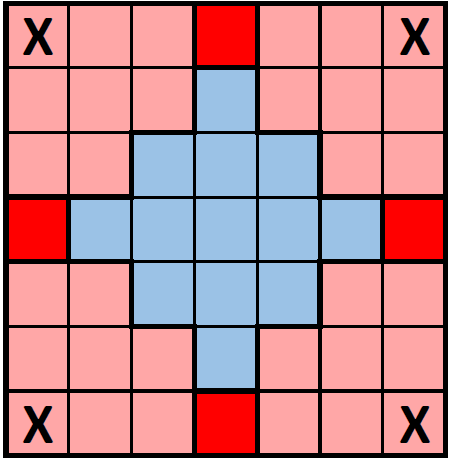
\includegraphics[width=0.8\textwidth]{images/corolle_placement_finales}}
			\end{figure}
		\end{minipage}\hfill
		\begin{minipage}{0.47\textwidth}
			\begin{figure}
				\only<1>{\includestandalone[mode=image,width=\textwidth]{graphics/ouvertures}}
				\only<2>{\includestandalone[mode=image,width=\textwidth]{graphics/finales}}
			\end{figure}
		\end{minipage}\hfill
	\end{frame}
	
	\begin{frame}{Approche Incrémentale}{\textbf{Exemple :} Polybridge}
		\begin{figure}
			\only<2>{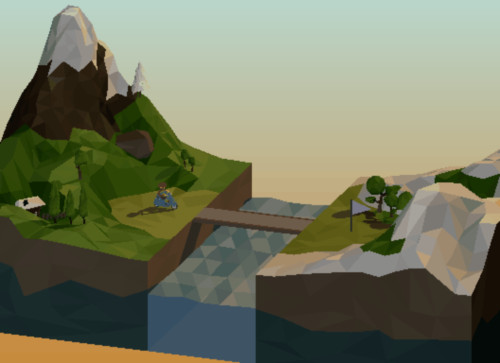
\includegraphics[width=0.7\linewidth]{images/polybridge_level_1}}
			\only<1>{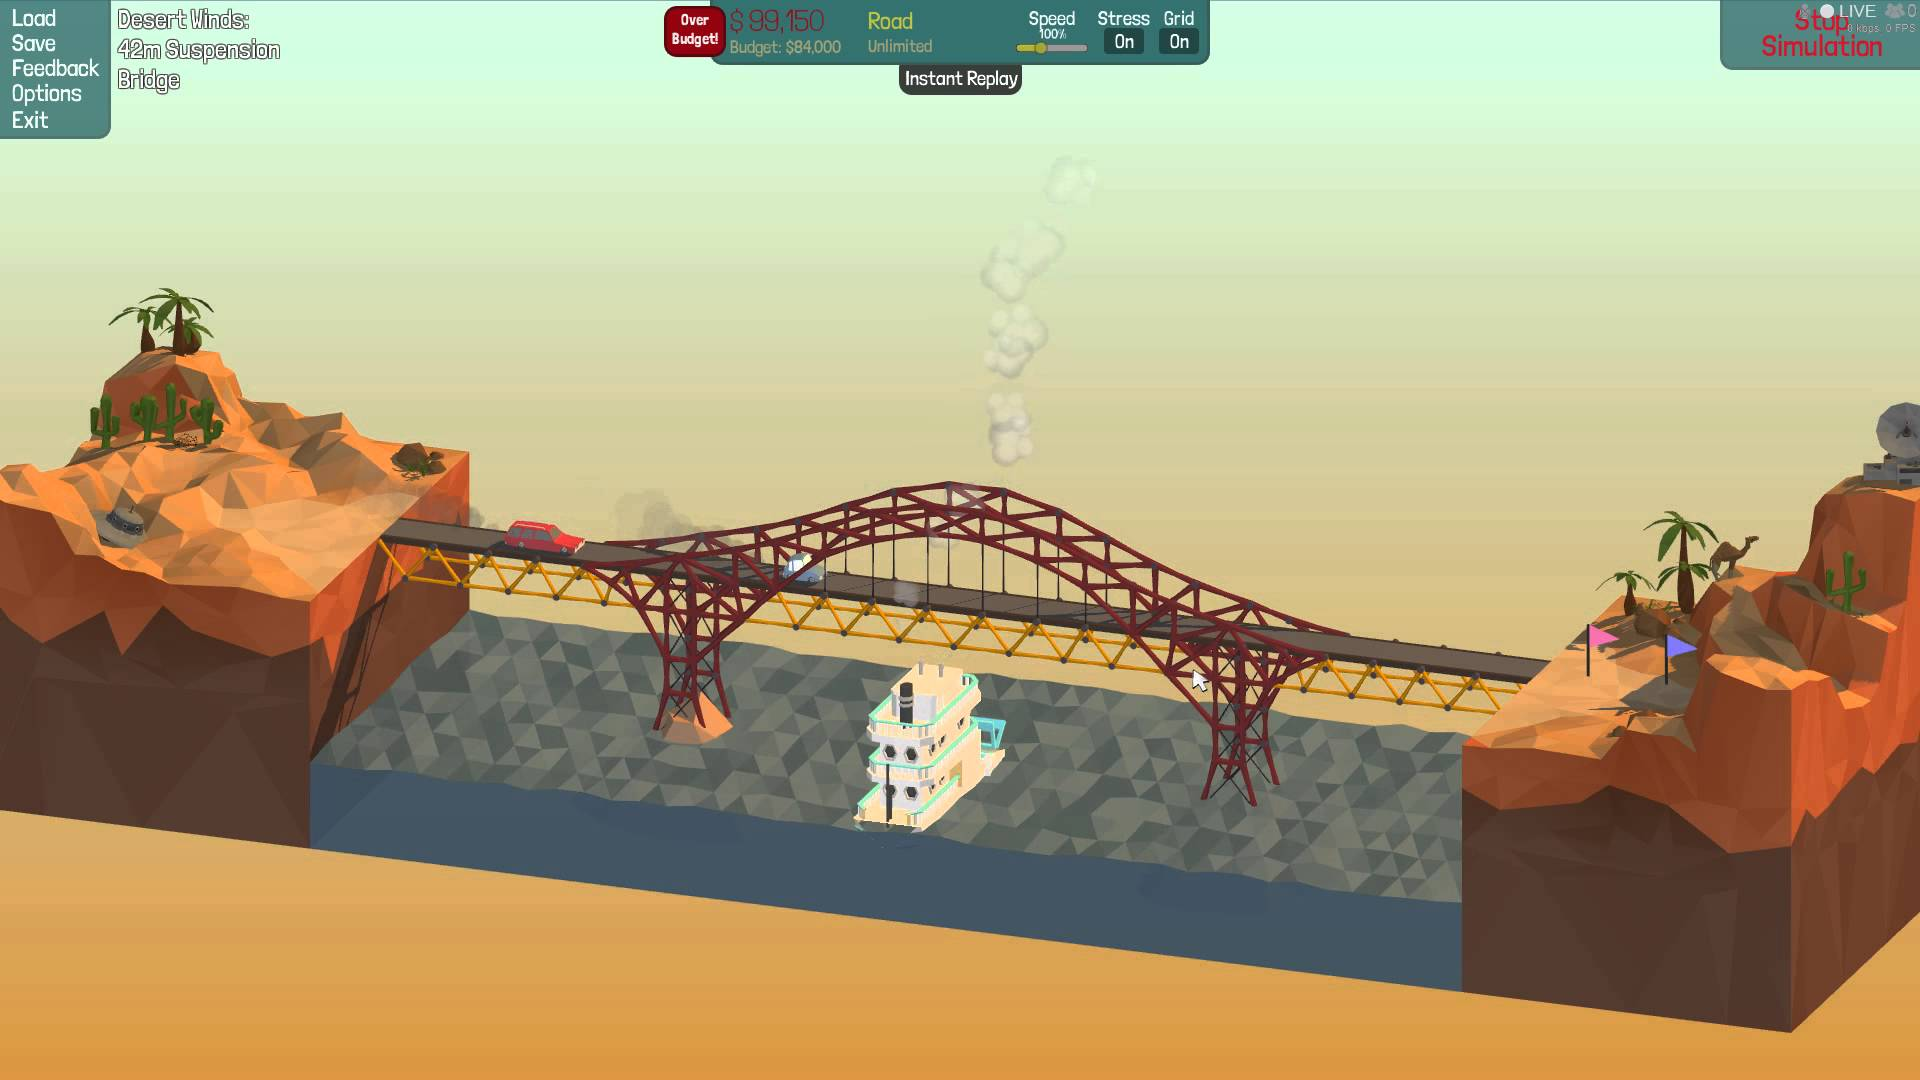
\includegraphics[width=\linewidth]{images/polybridge_level_3}}
		\end{figure}
	\end{frame}

	\subsection{Bruteforce et Smartforce}
	\begin{frame}{Principe}
		\begin{Bblock}{Bruteforce}
		\begin{itemize}
			\item Établir des valeurs étalons
			\item Valider des stratégies de parcours
		\end{itemize}
		\end{Bblock}
		\begin{Vblock}{Smartforce}
			\begin{itemize}
				\item Augmenter la quantité d'information
				\item Réduire la taille de l'espace à énumérer
			\end{itemize}
		\end{Vblock}
	\end{frame}
	
	\subsection{Corolles}
	\begin{frame}
		\begin{itemize}[<+->]
			\item Pré-calculer des patterns ou formes admissibles
			\item Utile pour les ouvertures et les finales
			\item Mises à jour dynamiquement
		\end{itemize}
		\begin{minipage}{0.47\textwidth}
			\begin{figure}
				\only<1>{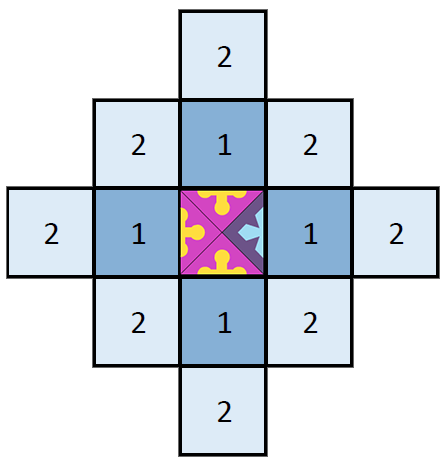
\includegraphics[width=\textwidth]{images/corolle_piece}}
				\only<2->{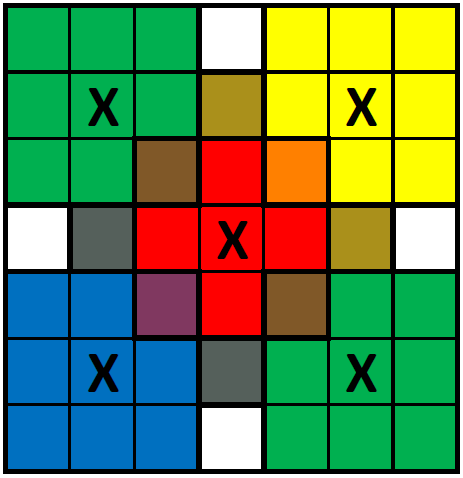
\includegraphics[width=\textwidth]{images/corolle_placement}}
			\end{figure}
		\end{minipage}\hfill
		\begin{minipage}{0.47\textwidth}
			\begin{figure}
				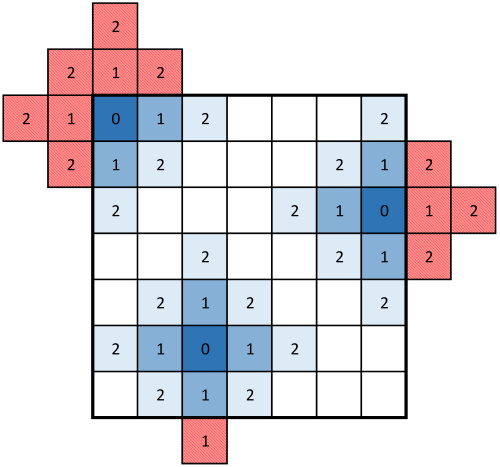
\includegraphics[width=\textwidth]{images/corolle_formes}
			\end{figure}
		
		\end{minipage}\hfill

	\end{frame}
	
	\subsection{GPU}
	\begin{frame}{Différence entre GPU et CPU}
		Le nombre total de corolles différentes de hamming 2
		\begin{itemize}
			\item pour un plateau $6\times 6$ : \textbf{317}
			\item $7\times 7$ : \textbf{804}
		\end{itemize}
		\begin{minipage}[t]{0.47\textwidth}
			\begin{Bblock}{CPU \\Central Processing Unit}
				\begin{itemize}
					\item<1-> peu de c\oe urs logiques
					\item<2-> spécialisé dans les calculs complexes : $4353764\times 123523464$
				\end{itemize}
			\end{Bblock}
		\end{minipage}\hfill
		\begin{minipage}[t]{0.47\textwidth}
			\begin{Bblock}{GPU \\Graphics Processing Unit}
				\begin{itemize}
					\item<1-> beaucoup de c\oe urs
					\item<2-> spécialisé dans les calculs simples : $1+2$
				\end{itemize}
			\end{Bblock}
		\end{minipage}\hfill
	\end{frame}

